
\section{Introduction} \label{sec:Introduction}

It is generally agreed upon that large-scale, universal quantum computing will require comprehensive error correction \cite{Wang2011,Fowler2012}.





There has been a recent proposal to make use of dopants in silicon to act as qubits \cite{the paper} to implement a version of the surface code. 


We have simulated a probe qubit interacting with four data qubits. The probe qubit is performing a circular orbit $40$ nm above the data qubits, and in this document we will document the effect of various errors. These errors include dephasing, dopan placement uncertainties and a path jitter. 


\subsection{The surface code}
The surface code is one of the most-well studied fault-tolerant codes \cite{something}. Its versatility, large code distance and large fault-tolerance threshold have contributed to various proposals \cite{some review} and some attempts at physical implementation \cite{Martinis?}. One key aspect of the surface code is its use of vertex and plauette operators that perform stabiliser measurements on four data qubits at a time. If the stabiliser gives a measurement outcome $-1$, it means that the four data qubits contain an error, whereas a $+1$ outcome indicate that the qubit states are in the codespace. As a consequence, the stabiliser measurements cannot identify errors that correspond to logical operations. At the same time, the stabiliser allow us to actually perform logical operations, which means that a physical implementation of the surface code would not require individual addressing of the data qubits. 

The stabilisers measurements themselves are performed by letting the data qubits interact with one single probe qubit. The probe qubit is the measured, and its outcome tells us about the parity of the measurement, that is, whether none or two,  (even parity) one  or three (odd parity) errors have been detected. Of course, the stabiliser measurement can also fail, but this is taken into account in large-scale fault-tolerance calculations. 




\subsection{A physical implementation}
In a paper in 2015, it awas proposed by G'Orman \textit{et al}. proposed a scheme for implementing the surface code in silicon \cite{the paper}.  To perform the stabiliser measurements, a probe qubit of a different dopant species is placed on a mobile slab above the data qubits. 

The data qubits are dopants placed in silicon placed in a square pattern using the best dopant placement techniques available, which currently stand at [insert some error value and cite it].

Each probe qubit performs a stabiliser measurement on four data qubits, a procedure which is performed by physically moving the overhead slab with the probe qubits. 



\begin{figure}[H]
	\centering
	\subfloat[]{ 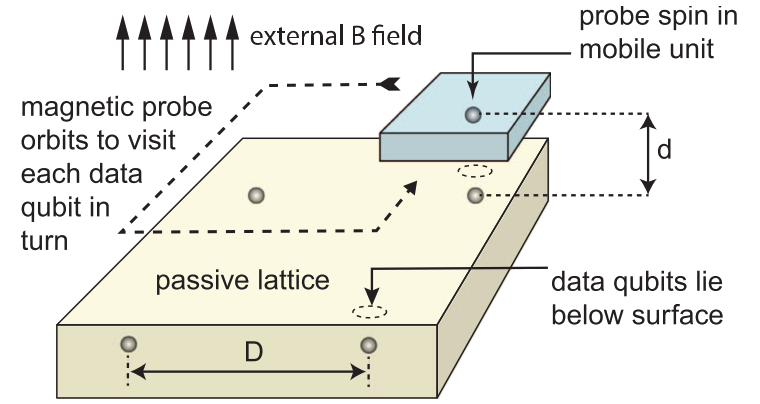
\includegraphics[width=0.8\linewidth]{../Figures/paper-parity} \label{FIG:paper-parity}}\\
	\subfloat[]{ 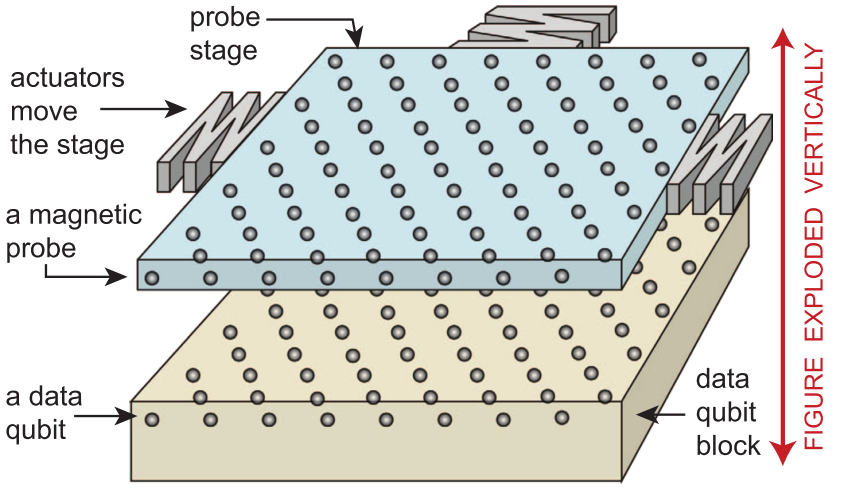
\includegraphics[width=0.8\linewidth]{../Figures/paper-mems} \label{FIG:paper-mems}}
	\caption[oddeven]{}
	\label{FIG:paper}
\end{figure}

The orbit can be performed in two different wasys: either through an abrupt orbit, where the probe qubit is moved rapidly from one data qubit to another, or through a smooth, circular orbit which brings the probe qubit directly on top of each of the data qubits. 

In Figure \ref{fig:thresholds} we see a large-scale fault-tolerance simulation which accounted for a large number of errors. Several thresholds were obtained, either for the abrupt or the circular orbit, and with respect to the data qubit placement accuracy. In each graph, the nature of the displacement is shown as either a `pillbox' or an ellipsoid shape. They found reasonable thresholds for each configuration, which shows that the general principle of this setup is valid. 

If we were to implement such a system in the lab, we would probably start with the smallest possible building block, which in this case is the system consisting of four data qubits and 

For each parameter configuration. 

